\documentclass[conf]{new-aiaa}
%\documentclass[journal]{new-aiaa} for journal papers
\usepackage[utf8]{inputenc}
\usepackage{import}
\usepackage{hyperref}
\usepackage{graphicx}
\usepackage{amsmath}
\usepackage[version=4]{mhchem}
\usepackage{siunitx}
\usepackage{longtable,tabularx}
\usepackage{placeins}
\usepackage{transparent}
\usepackage{pdflscape}
\usepackage{afterpage}
\usepackage{tablefootnote}
\setlength\LTleft{0pt}
\usepackage[table,xcdraw]{xcolor}
\usepackage{natbib}
\graphicspath {{figures/}}


\usepackage{subcaption}


\usepackage{subcaption}
\usepackage{booktabs}
\usepackage{float}
\usepackage{multirow}
\usepackage{geometry}
\usepackage{amsfonts}
\usepackage{amssymb}
\usepackage{tikz}

\usetikzlibrary{arrows,chains,positioning,scopes,shapes.geometric,shapes.misc,shadows}


\usepackage{array}
\newcolumntype{L}[1]{>{\raggedright\let\newline\\\arraybackslash\hspace{0pt}}m{#1}}
\newcolumntype{C}[1]{>{\centering\let\newline\\\arraybackslash\hspace{0pt}}m{#1}}
\newcolumntype{R}[1]{>{\raggedleft\let\newline\\\arraybackslash\hspace{0pt}}m{#1}}


\setlength\LTleft{0pt}

\title{EECS 587 Project: Parallel-in-time algorithms for system sensitivities}
\author{Josh Anibal}
% \author{Charles A. Mader\footnote{Research Investigator, AIAA Senior Member}}
% \affil{University of Michigan, Ann Arbor, Michigan}

\begin{document}

\maketitle


% Notes
% - unsteady problems are of interest
%    - active flow control
%    - acoustics

% time averaged objective function





% unroll coupled loops?



% \section{Nomenclature}

% {\renewcommand\arraystretch{1.0}
% \noindent\begin{longtable*}{@{}l @{\quad=\quad} l@{}}
% $A$  & amplitude of oscillation \\
% \end{longtable*}}




\begin{abstract}

    Gradient-based-optimization is ideal for engineering design optimization problems, which typically have a large number of design variables.
    However, gradient-based-optimizers require sensitivity information to drive the objective function to a minimum.
    Even if analytical methods are used, sensitivity routines can be a bottleneck for large engineering models or when coupled analyses are used.


    % This is similar to backward propagation for neural networks except a linear system may need to be solved for each step making some steps more expensive and the process must be repeated for each objective and constraint.

    % Because there are typically more design variables than functions of interest, model sensitivities are calculated in the reverse mode.
    In forward mode differentiation, the inputs of one analysis's sensitivity routine are provided by the outputs of sensitivity routines earlier in the execution order.
    The same is true for reverse mode differentiation, but the execution order of the sensitivity routines is the opposite of the model execution order.
    Because each sensitivity routine only depends on results of prior routines, there is a time-like dependency structure between sensitivity routines.

    Parallelizing tasks with a time-like dependency structure is non-trivial, but will become increasingly important to achieve good performance as computer architectures become increasingly concurrent.
    It is for this reason we propose using algorithms developed for parallel-in-time execution to parallelize the computation of sensitivities for engineering models.
	To study the effectiveness of these algorithms for such a purpose we first applied a modified version of the algorithm Parareal to a representative problem and analyzed its scaling behavior.
	In these studies we found the algorithm used had poor scaling and a maximum speedup of only 1.5 times.
	These poor scaling properties leads us to the conclusion that the parallel-in-time algorithm Parareal was not found to be an effective way to speed up the calculations of sensitivities in engineering models.
	% In this work we will highlight any gains in performance from the execution of parallel-in-time sensitivity analysis for a low-fidelity heat-transfer constrained design problem. % or an aerostructural problem?
    % We will do this by implementing our engineering model and sensitivity analysis inside the open source optimization framework OpenMDAO \cite{Gray2019a}.



\end{abstract}





\section{Introduction}


% engineering models are complicated
Engineering models are composed of many sub-analyses.
For example, in aerospace engineering a model to predict the fuelburn of an aircraft may be composed of analyses to compute geometry, aerodynamic performance, structural stresses, engine performance, and trajectory.
Each of those analyses may be coupled with an other analyses and many consist of many more sub-analyses.

Despite there complexity, optimization frameworks, such as OpenMDAO\cite{Gray2019a}, make it easy for engineers to construct models by defining components for each analysis and then connecting components to form models.

The open source tool OpenAerostruct\cite{Jasa2018a} provides an example of such models.
Figure \ref{fig:n2} shows the top level components of an OpenAerostruct model in an N2 diagram where the components are aligned on the diagonal and the off diagonal terms show the connections between models.


\begin{figure}[H]
	\centering
	\includegraphics[width=0.6\textwidth,keepaspectratio]{n2.png}
	\caption{The N2 representation of this OpenAerostruct shows the components on the diagonal}
	\label{fig:n2}
\end{figure}

The components of this model are composed of even more sub-components.
Figure \ref{fig:n2_exp} attempts to show the N2 representation with all 62 of the sub-components exposed.

\begin{figure}[H]
    \centering
    \includegraphics[width=0.6\textwidth,keepaspectratio]{n2_exp.png}
	\caption{N2 representation of an OpenAerostruct model with all the sub-components exposed}
	\label{fig:n2_exp}
\end{figure}


% optimization uses models
To use a engineering model, such as the OpenAerostruct model, in large scale design optimization one needs to write sensitivity routines for each component.
For an component that solves PDEs this may involve using the adjoint or the direct method.
Using the Unified Derivative Equation\cite{Martins2013a}, which is a generalization of the chain rule, the sensitivity routines of each component can be combined to get derivatives of objective functions and constraints with respect to the design variables.
Derivatives can be calculated in this way in both the forward or reverse mode.

% either way the sensitivity routines have time dependency structure
In the forward mode the each sensitivity routine is only influenced by those that came before in the model execution order and in the reverse mode each routine is only affected by those that come after.
In either sensitivity mode, the dependency of the routines is one way.

% this structure is common
This one-way dependency structure is very similar to that of a time-accurate simulation where each time step is only influenced by those that came before it.
Because this type of simulation is so common, research effort has already been applied to parallelize these simulations in time despite the difficulty inherent to the dependency structure.

% work has been done on this problem
Gander\cite{Gander2015} provides a review of this work and showcases key contributions.
The author of the review highlights the recent increased interest in parallel-in-time algorithms now that processor clock speeds have plateaued.
The current trend in computing is toward using increased parallelism to provide increased performance.
This trend is unlikely to reverse anytime soon especially as GPUs find there way into mainstream computing and we move into the exascale era.

% people are applying this work else where
Because of the rising importance of parallelism, recent work has been done to apply the research on algorithms for parallel time accurate simulations to problems with the same structure.
Gunther et al.\cite{Gunther2019} have shown that the parallel-in-time algorithm MGIRT\cite{Falgout2014} was effective at reducing the computational time required to solve for sensitivities of an unsteady adjoint problem.
Furthermore, Gunther et al.\cite{Gunther2020} have applied the same technique to speedup back-propogation for neural networks and shown its effectiveness.


% this hasn't be applied to general engineering models yet
At present no work has been done to parallelize the execution of sequential sensitivity routines within the sensitivity computations for engineering models.
The aim of this work is to address this absence by applying parallel-in-time (PinT) algorithms to this task and highlighting the performance enhancements.


\section{Problem}
To explore the idea of using PinT algorithms to speed up sensitivity calculations we first need a problem to test our algorithm on.
Since this study is exploratory a suitable problem should be rather basic.
However, it must also be scalable so that we may fully test the algorithm.

To stratify these requirements our model will consist of N identical components connected in series and is shown schematically in Figure \ref{fig:model}.
In this model each component only passes values to the component ahead of it and only receives values from the component behind it.
Similarly when calculating sensitivities in the reverse mode, the derivative seeds are propagated backwards from the last component to the first.

\begin{figure}[H]
	\centering
	\includegraphics[width=0.90\textwidth,keepaspectratio]{model.png}
	\caption{A schematic view of the problem used in this study}
	\label{fig:model}
\end{figure}


Although, this problem represents a vary simple dependency structure between components it incorporates the key difficult in computing sensitivities; passing information all the way from one side of the model to the other.
Within each component a linear system will have to be solved to calculated the derivative seeds of the inputs.
This represents a case where the components calculate their outputs by solving an implicit equation, which is the case for models based on PDEs.

It is important that the system that is being solved by each component has the same same structure as a real problem.
This is because it has been shown that PinT algorithms can have a different effectiveness for matrices which represent different physical problems.
As a result the matrix was carefully chosen.
The matrix was take from a component constructed to solve a steady aeroelastic analysis in OpenAerostruct.
The component uses a vortex lattice method to calculate loads at points along the wing and a beam model to calculate the subsequent deflections
By chaining this component together it represents a model similar to a quasi steady aeroelastic analysis.
The matrix represent the jacobian of the state variables of the system with respect to the residuals.
By varying the finest of the discretization we can create matrices of varying size.
Using this method 417x417, 2387x237, 21830x21830, 90711x90711, 342711x342711 matrices were created.




\section{Algorithm}

The algorithm used to parallelize the sensitivity calculation is based on the parareal algorithm.
Parareal is one of the most popular PinT algorithms and has a wide body of literacy describing its implementation and performance properties.
% describe what the parareal algorithm is

% decompose the time
To use Parareal, the time domain must be decomposed into as many sum domains as the number of processors, $P$.
For our sensitivity propagation problem, the domain is the collection of all the models components.
Thus the sub domain are formed by creating subsets of the the model components as shown in Figure \ref{subdomains}


\begin{figure}[H]
	\centering
	\includegraphics[width=0.90\textwidth,keepaspectratio]{subdomains.png}
	\caption{The sub domains needed for the Parareal algorithm are formed by taking sub sets of the model components}
	\label{fig:subdomains}
\end{figure}


Each processor will work towards solving the problem on its sub domain.
This is done by preforming iterations using a \emph{coarse} and a \emph{fine} methods for solving the problems on the sub domains.
As the names suggest, the coarse method should supply an approximate solution to the problem at low cost, while the fine method should supply an arcuate answer to the problem at a much higher cost.

For our sensitivity propagation problem, the fine method will be an accurate solve of the linear system of each component while the coarse method is an inexact solve of the same system.
For both methods the iterative solver GMRES will be used but with different tolerances.
The fine solver has a tolerance of 1e-9, which is the smallest tolerance that could be reliably solved, while the coarse method has a tolerance of 1e-5.




The algorithm is initialized by computing a coarse solution to the problem by using sequentially using the coarse solution method on each sub domain.

\begin{equation}
    y_{j+1}=\mathcal{G}\left(y_{j}, t_{j}, t_{j+1}\right), \quad j=0, \ldots, P-1
\end{equation}


Then in parallel each processor computes the solution of the fine problem based on an initial condition of the sub domain using the coarse solution
\begin{equation}
    y_{j+1}=\mathcal{F}\left(y_{j}, t_{j}, t_{j+1}\right), \quad j=0, \ldots, P-1
\end{equation}


A sequential correction is then made based on the fine solution and the difference in coarse solution at current and prior iteration.


\begin{equation}
    y_{j+1}^{k+1}=\mathcal{G}\left(y_{j}^{k+1}, t_{j}, t_{j+1}\right)+\mathcal{F}\left(y_{j}^{k}, t_{j}, t_{j+1}\right)-\mathcal{G}\left(y_{j}^{k}, t_{j}, t_{j+1}\right), \quad j=0, \ldots, P-1, \quad k=0, \ldots, K-1
\end{equation}

Parallel fine solutions and sequential corrections are performed iteratively until the the solution across the entire time domain converges.
Because The parallel algorithm  executes all fine solutions in parallel, it is a PintT algorithm that is categorized as a parallel across the steps method.
It can be shown that the parareal algorithm will converge to the exact solution in the general case in P iterations or less.
However, if the algorithm converges in P iterations no speed up will be achieved.
Thus to achieve meaningful speedups with the basic algorithm it must converge in far fewer than P iterations.



To further improve on the basic algorithm, the prior corrected solution can be used as an initial guess for the fine method and the prior coarse solution can be used as an initial guess for the coarse method.
It is import not to use the current corrected solution as the initial guess for the coarse method as this will cause the algorithm to converge to the incorrect answer.
This technique requires additional memory to save the prior solution, but reduces the cost of the next iteration.

Another modification made to the original Parareal algorithm was to skip fine solutions and corrections on sub domains which have already converged to the exact solution.
Because sub domain $j $ where $j$ is $0 < j < P$ will converge to the exact solution after $j$ iterations there is no need to update it in future iterations.
By skipping the update of those sub domains in the sequential correction and parallel fine solve step, we reduce the cost of each as the algorithm progresses.
These two optimizations lead to a faster algorithm overall than the original Parareal algorithm.



\subsubsection{Parallelsim}
This algorithm can be parallelized using either shared memory or distributed memory.
For this project MPI was used to incorporate distributed memory parallelism.
Distributed memory parallelism was chosen because the solution methods used on each sub domain may require solving large systems that require lots of memory.
As a result the algorithm may need to be run on multiple nodes.
MPI and distributed memory parallelism provides a flexible solution for supporting inter and intra node parallelization.

At each iteration of the algorithm messages are pasted backwards between subdomains during each sequential solve.
blocking communication is used to prevent the processor from moving forward until it has the information it needs to do so.
No barriers are used to allow greater overlap in computation.
Figure \ref{fig:overlap} shows the ideal case of parallel execution. it was found that load balancing was necessary to achieve this.


\begin{figure}[H]
	\centering
	\includegraphics[width=0.80\textwidth,keepaspectratio]{overlap.png}
	\caption{The algorithm used always for the subdomains to overlap calculations}
	\label{fig:overlap}
\end{figure}



\subsubsection{Load balancing}
It was found that equally distributing the components of the model across processors was not ideal.
For our particular problem it was discovered that components that that were closer to the end took more time to solve both fine and coarse problems.
This was a major issue because during the sequential update all processor downstream need to wait until the prior processor has completed it's sequential update.
To ensure the processors were not holding up later processors, the earlier processors were given less work.


However, this load balancing technique required prior knowledge about how long each linear system would take to solve.
Estimation of the time needed to solve the linear system on each component before trying is is hard to solve in general.
One could use the condition number or eigenvalues of the matrix to estimate how difficult it will be to solve a system of that size.
However, these are expensive to compute and in this example even though all of the components use the same matrix the time to solve still differed by a factor of up to 8.

\section{Results}

To test the scalability of the algorithm both strong and weak scaling tests were performed.
The strong scaling study was performed on a single node of the GreatLakes computing cluster using two 3.0 GHz Intel Xeon Gold 6154 processors.
The weak scaling study was performed on a desktop computer using a 4.00GHz Intel i7-4790K processor.



\subsection{strong scaling}
The strong scaling tests revealed that the algorithm had a maximum speedup up 1.5x when run in parallel.
Figure \ref{fig:speedup} shows the speed up achieved as the number of processors increases.
The peak speedup of 1.5x occurs at 4 processors, and decreases to a speedup of less than 1 with 32 processors.

\begin{figure}[H]
	\centering
	\includegraphics[width=0.60\textwidth,keepaspectratio]{strong_scaling.pdf}
	\caption{}
	\label{fig:speedup}
\end{figure}

This performance result is disapointing and thought about why this is the case are discussed in the Discussion section.



\subsection{weak scaling}

Similarly, the weak scaling of the algorithm is poor as shown by Figure \ref{fig:weak_scaling}.
As the number of processors are increased the size of the problem is increased as well at the same rate.
To increase the problem size the number of components in the model is doubled when the number of processors is also doubled.
This was done for the three largest matrix sizes to study how it might affect the scalability.


% \begin{figure}[H]
% 	\centering
% 	\includegraphics[width=0.60\textwidth,keepaspectratio]{weak_scaling.pdf}
% 	\caption{}
% 	\label{fig:speedup}
% \end{figure}
\begin{figure}[H]
	\centering
	\includegraphics[width=0.60\textwidth,keepaspectratio]{weak_scaling.pdf}
	\caption{}
	\label{fig:weak_scaling}
\end{figure}

Help by the fact that the added component tended to be easier to solve as mentioned in the load balancing section.



\section{Discussion}

\subsection{Usefulness}

The maximum speed up in the calculation of sensitivities from using a parallel in time algorithm was not large enough to be great partial use.
It is often the case that there is a better way to speed up the sensitivity analysis of each component by using parallelism.
For cases where the sensitivities calculations require solving a linear system like in our example problem, then one would be better off using parallel iterative solver.
Such solvers are we established and are included in libraries such as PETSC where they have been shown to have good scalability up to many thousands of corse.

The value of the algorithm would be to add auxialiary option for parallelization when the individual component themselves cannot be parallelized or already been parallelized to the maximum extend possible.

One case where the components themselves may be hard to parallelize is were they represent simple functions like in a neural net work.
Another case where this algorithm may be useful is if one was using a truly massive model where different componets resided on different comput nodes in order to have sufficent memory.
In this case, with the proposed algorithm all nodes could at least do some useful work instead of having some sit idle.

\subsection{Explanation}



Parallelization in time is inherently difficult.
Unlike parallelization in space where nodes depend on only spacial neighbors, In time parallelization nodes depend on all previous nodes.
As a result you cannot simply split the domain and correct cells near the interface; corrections must be propagated through all nodes ahead in time.


Regardless of this difficulty algorithm such as parareal attempt to parallelize problems in time anyway.
However, the success of these algorithms is limited.
For an algorithm like parareal, a 60x speedup with 500 cores is considered a good result.
This is because the parareal algorithm speed up is bounded by the inequality given in equation \ref{eqn:speedup}.


\begin{equation}
    S_{p}=\frac{c_{\text {fine }}}{c_{\text {parareal }}}=\frac{1}{(K+1) \frac{N_{c}}{N_{f}} \frac{\tau_{c}}{\tau_{f}}+\frac{K}{P}} \leq \min \left\{\frac{N_{f} \tau_{f}}{N_{c} \tau_{c}}, \frac{P}{K}\right\}
    \label{eqn:speedup}
\end{equation}

To maximize our achievable speedup we need a K << P and a coarse method which is much faster than the fine method.
It may not be obvious at first, but these two objectives are in competition with one another.
To achieve a small number it iteration K, more accurate updated must be used at each iteration.
This requires a coarse method that is more accurate and thus more costly.
So, with all else being held equal to decrease the term $\frac{P}{K}$ one must increase the term $ \frac{N_{f} \tau_{f}}{N_{c} \tau_{c}} $.
Thus the maximum speedup of the parareal algorithm is limited by a compromise between both terms.



although our algorith is differernt than the basic parareal algorithm, the modifications are only minor and therefore it is still useful to consider speedup properties of the parareal algorithm.

For our problem the cost of the coarse and fine methods are determined by the tolerances use for the linear solver.
In general, the error of iterative linear solvers converge linearly with the number of iterations.
gmres converges linearly.

\begin{figure}[H]
	\centering
	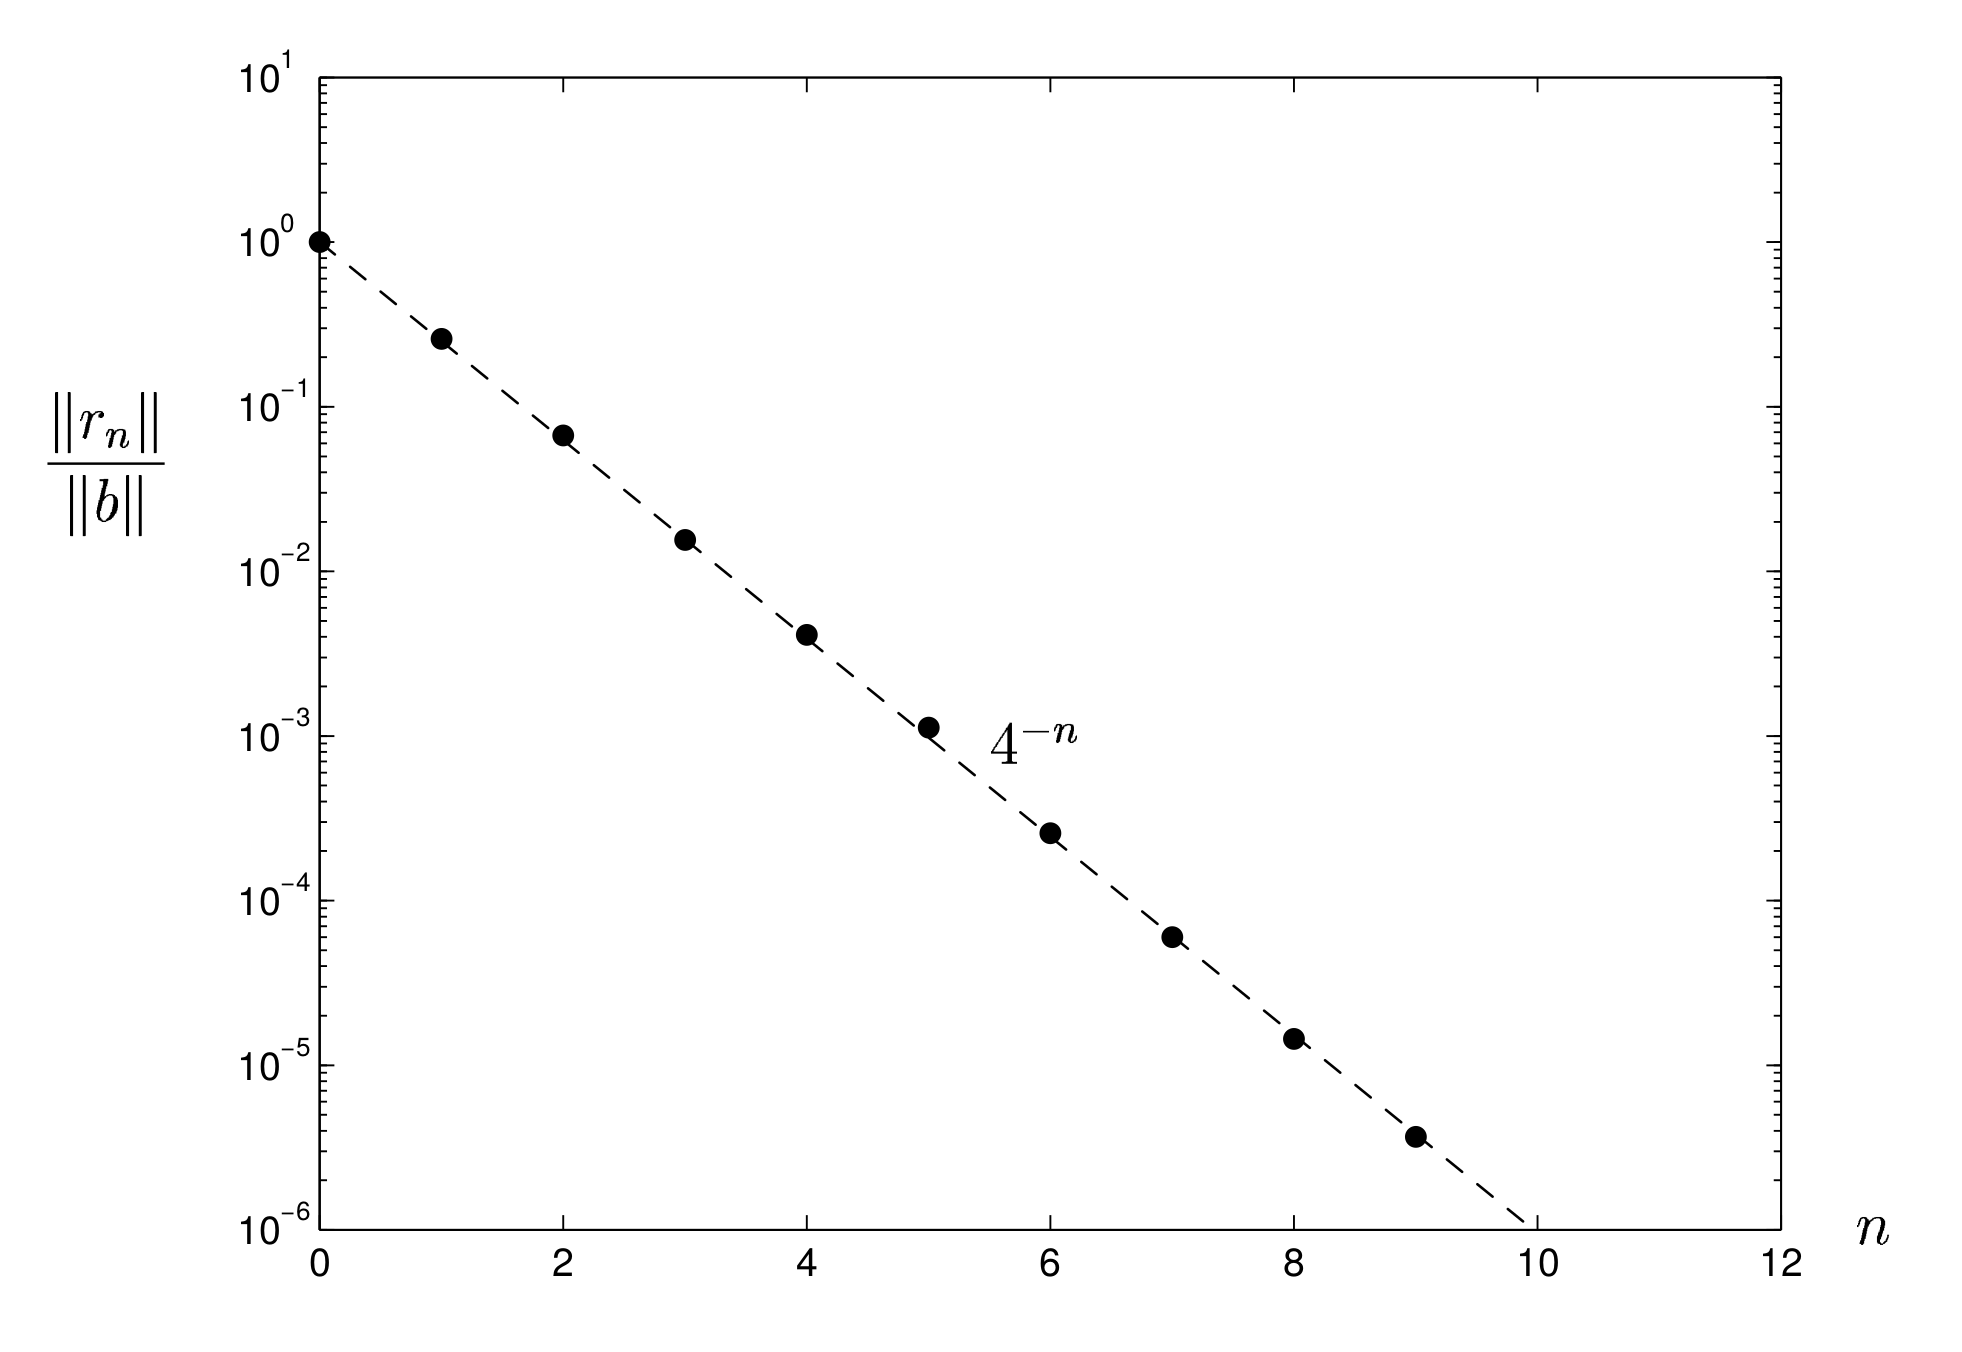
\includegraphics[width=0.60\textwidth,keepaspectratio]{gmres_conv.png}
	\caption{Convergence rate of GMRES for a well behaved matrix from "Numerical Linear Algebra" by Trefethen and Bau}
	\label{fig:gmres_conv}
\end{figure}

Since the cost per iteration is constant then the cost also scales linearly.




we can confirm this by analying the solution time need to solve the matrices used to certain tolerance.
Figure \ref{fig:acc_timing} indeed shows that as the solver tolerance increases the cost to solve each matrix increases approximately linearly

\begin{figure}[H]
	\centering
	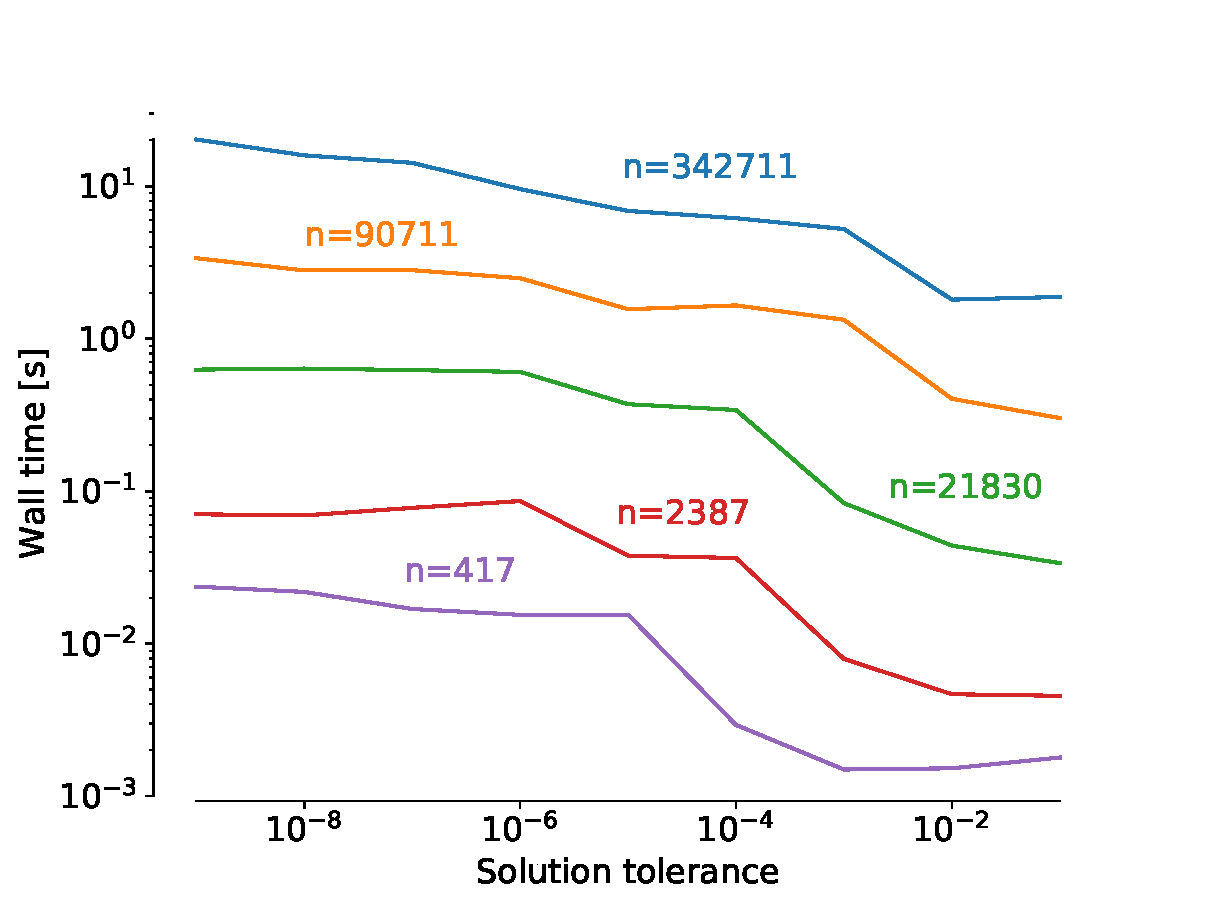
\includegraphics[width=0.60\textwidth,keepaspectratio]{acc_timing.pdf}
	\caption{The cost to solve each matrix using GMRES for a given level of accuracy}
	\label{fig:acc_timing}
\end{figure}

Pretty remarkable, but it means that a pure parareal algorithm the max speedup is at most 2x for the levels of fine and coarse solvers used.
- For twice as many orders of accuracy the cost of the solution only doubles.
solver tolerance off 1e-5 and 1e-9 were found to produce the greatest speed up
for a basic parareal algorith this would limit the speed up to 1.8x




maybe the method of submatrices and use a GPU




In addition to the low ratio of fine cost to coarse cost, it was found that the solution would not converge in less than P iterations for our problem.
Figure \ref{fig:res_hist} shows the error in the solution after each iteration at different points in time.
Although the figure is shown for the particular case with 8 processor and the 90711x 90711 matrix it is representative of the other cases aswell.

\begin{figure}[H]
    \centering
    \includegraphics[width=0.60\textwidth,keepaspectratio]{res_hist.pdf}
    \caption{}
    \label{fig:res_hist}
\end{figure}


- It could be we simply didn't have the right types of matrices for the parareal algorithm to be effective


It is not fully understood why this happened, although the equation for the converge of error by parareal, Equation \ref{eqn:conv}, gives us a clue. The variables that are important in that equation are $k$, the number of iterations, and $N$, the number of sub-interval.

\begin{equation}
	\max _{1 \leq n \leq N}\left|u\left(t_{n}\right)-U_{n}^{k}\right| \leq \frac{\left(C_{1} T\right)^{k}}{k !} e^{C_{2}(T-(k+1) \Delta T)} \Delta T^{\rho k} \max _{1 \leq n \leq N}\left|u\left(t_{n}\right)-U_{n}^{0}\right|
	\label{eqn:conv}
\end{equation}

There are many factors in the right hand side of Equation \ref{eqn:conv}, but the one that is most important is $\frac{\left(C_{1} T\right)^{k}}{k !}$.
Eventually, $k!$ will grow faster than $\left(C_{1} T\right)^{k}$, but his may not happen until k is very large.
Thus to achieve converge before P iteration, P must be sufficiently large to allow enough iteration for the $1/k!$ factor to dominant.
However, for our problem even 32 sub-intervals was not enough for the $1/k!$ factor to converge the error before P iterations.
Therefore to achieve any speedup at all we had to modify the basic parareal algorithm.
By reusing information we can make the cost of additional iterations cheaper, but with only small tweaks we can't do much better than the original parareal algorithm which has no speed up for this problem.

\section{conclusion}


The calculation of engineering sensitivities are a bottle neck in design optimization.
In an attempt to speedup this process we investigated the use of a modified version of the parallel-in-time algorithm Parareal to parallelize the problem.
We applied this algorithm to example models created by repeating a matrix from a real engineering problem.
The algorithm uses MPI to pass data about intermediate solution states to components on other processors.
By applying some load balancing to the problem the algorithm achieves better performance by reducing the time the processors are waiting to receive data.
The studies of the strong and weak scaling reveals that the algorithm does not scale well.
The algorithm works best with 4 or less processors and was only able to achieve a maximum speed up of 1.5x.
In conclusion, the use of the parallel-in-time algorithm parareal was not found to be an effective way to speed up the calculations of sensitivities in engineering models.
Analysis of the basic parareal algorithm provides some insight into the theoretical limitations that may have contributed to the poor performance of the modified version of parareal we used.




\bibliography{mybib,mdolab}

\end{document}
